\section{Introducción}
\label{cap:introduction}

\subsection{Contexto}
\label{sec:context}


El estudio evolutivo de un grupo de organismos es esencial en la biología para comprender la relación histórica de éstos a lo largo del tiempo. Aunque no es posible observar directamente la relación evolutiva, se pueden utilizar técnicas de estimación para proponer hipótesis que expliquen la evolución del grupo en estudio \citep{Warnow2017}. El análisis filogenético tiene diferentes aplicaciones en distintos campos de la ciencia, tales como medicina, biogeografía, química, epidemiología y paleontología, entre otros \citep{Morrison2012}. Dentro de las investigaciones más recientes se encuentra el estudio de la historia evolutiva del SARS-CoV-2, en donde se utilizó el análisis filogenético para aportar información respecto a la dinámica de transmisión y la importancia de tomar medidas de control para detener la propagación de la infección \citep{Castillo2020,Jaimes2020}. Es por ello que el análisis filogenético es una herramienta fundamental en la biología evolutiva, ya que utiliza evidencia biológica para inferir la relación entre los organismos y proponer hipótesis evolutivas que a menudo son representadas como árboles filogenéticos \citep{Carrio2018} (Figura \ref{fig:phyloTree}).

En un árbol filogenético, las hojas representan a las especies que están siendo estudiadas y los nodos indican el ancestro común más reciente. Las ramas del árbol representan las relaciones evolutivas entre los diferentes nodos, y la longitud de las ramas indican el grado de divergencia entre las especies o grupos de organismos. Estos árboles pueden ser clasificados como \textit{enraizados} o \textit{no enraizados}, esto dependiendo de la existencia o inexistencia de un ancestro común que indique la dirección de evolución. Por lo cual el número de posibles topologías a inferir es distinto dependiendo del árbol filogenético, sin embargo, en ambos casos la cantidad de topologías diferentes para el mismo conjunto de genes es de orden combinatorial. Es por ello que la inferencia filogenética ha sido clasificada computacionalmente como un problema \textit{NP-Hard} \citep{Felsenstein2004}.

\begin{figure}[hptb]
    \centering
    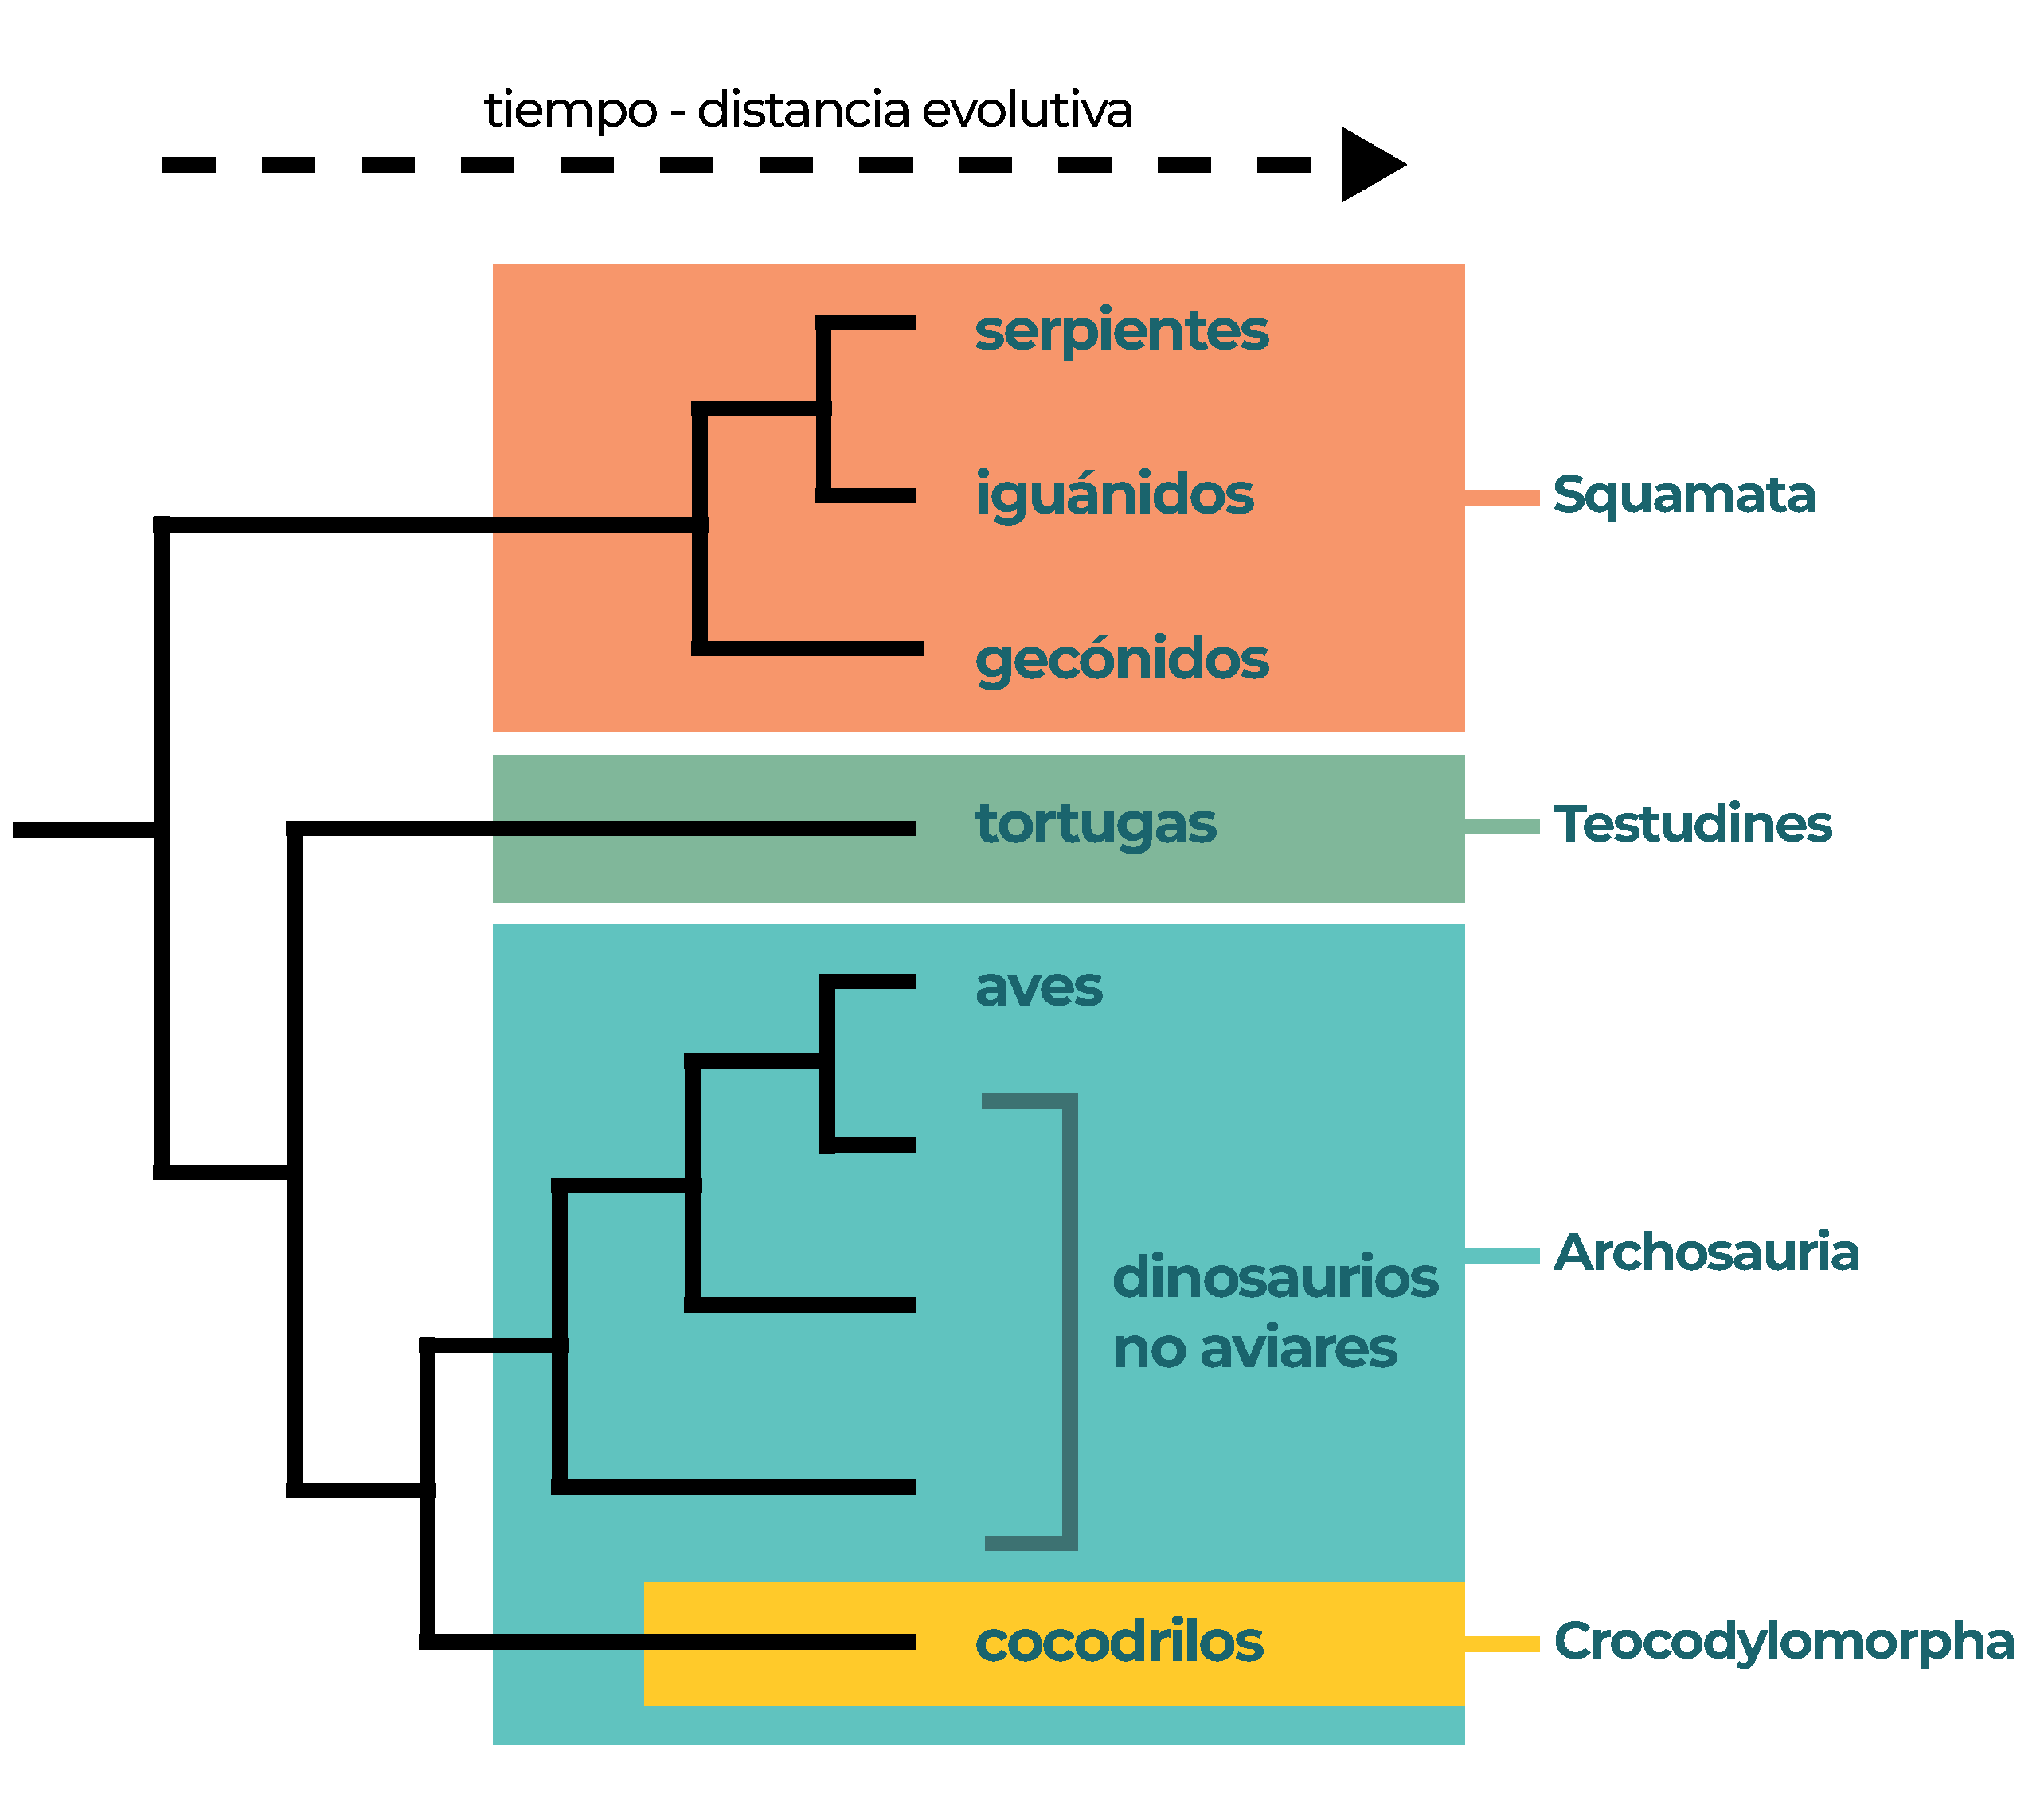
\includegraphics[scale=.24]{Images/phylogeneticTree.eps}
    \caption{Ejemplo de árbol filogenético adaptado de \citep{Irisarri2017}}
    \label{fig:phyloTree}
\end{figure}


En la literatura se han propuesto varios métodos para inferir árboles filogenéticos. Éstos se clasifican en aquellos que utilizan la distancia evolutiva como base y los que utilizan las características de los árboles como base para inferir. Entre los métodos basados en distancia evolutiva, se encuentras algunos que buscan soluciones aproximadas por medio de la optimización de una criterio en específico, tales como \textit{Mínima evolución} \citep{Kidd1971,Rzhetsky1993} o \textit{Mínimos cuadrados} \citep{Cavalli1967,Fitch1967}. Por otro lado, aquellos métodos que se basan en la características de los árboles comparan todas las secuencias alineadas, considerando la información de las características para calcular un puntaje para cada árbol generado. Esta categoría incluye \textit{máxima parsimonia, verosimilitud} y métodos bayesianos \citep{Vernygora2020}.

Al elegir un criterio para inferir un árbol filogenético, las topologías resultantes podrían estar sesgadas por éste, por las características de la data y modelo de evolución elegido \citep{VillalobosCid2018}. En los últimos años, se han propuesto diferentes enfoques de optimización multiobjetivo \citep{Handl2007} para lidiar con el problema de topologías sesgadas por un sólo criterio. Con ello se han obtenido mejores soluciones en términos de dominancia comparado con aquellos enfoques de optimización de un solo objetivo. Al momento de usar un enfoque multiobjetivo existe una  entre el espacio \textit{objetivo} y de \textit{decisión}. En donde el primero corresponde al espacio formado por las soluciones evaluadas por los criterios utilizados. Y el segundo espacio está compuesto por todas las topologías de árboles de la generación actual del algoritmo.




\subsection{Motivación}
\label{sec:motivation}


En la última década se han propuesto diferentes estrategias multiobjetivo para inferir árboles filogenéticos \citep{Santander-Jimenez2014,Santander-Jimenez2015,Santander-Jimenez2016,Santander-Jimenez2016b,VillalobosCid2018,Min2018,VillalobosCid2019,Zhang2020}. Sin embargo, estas propuestas convergen al aplicar estrategias elitistas que buscan optimizar los criterios en el espacio objetivos. Entre éstas se encuentra \textit{Crowding distance, Dominance level} y \textit{Hypervolumen indicator}.

A pesar de la utilización de estrategias que permitan optimizar los objetivos a evaluar durante la inferencia, las soluciones obtenidas por estos enfoques tienen un sesgo asociado al comportamiento de los dos espacios de trabajo (espacio de decisión y objetivo). Los resultados obtenidos en \citep{VillalobosCid2018c} sugieren que ambos espacios, en el contexto de inferencia filogenética multiobjetivo, no tienen una relación directa. Dando a entender que ambos son \textbf{sobreyectivos} pero no \textbf{inyectivos} (Figura \ref{fig:multimodalProblem}). Es decir, árboles con diferentes topologías pueden estar representados por el mismo punto sobre el espacio objetivo. Esto implica que los enfoques multiobjetivo pueden descartar soluciones de ciertas regiones del espacio de decisión, limitando así la diversidad de topologías inferidas.

\begin{figure}[hptb]
    \centering
    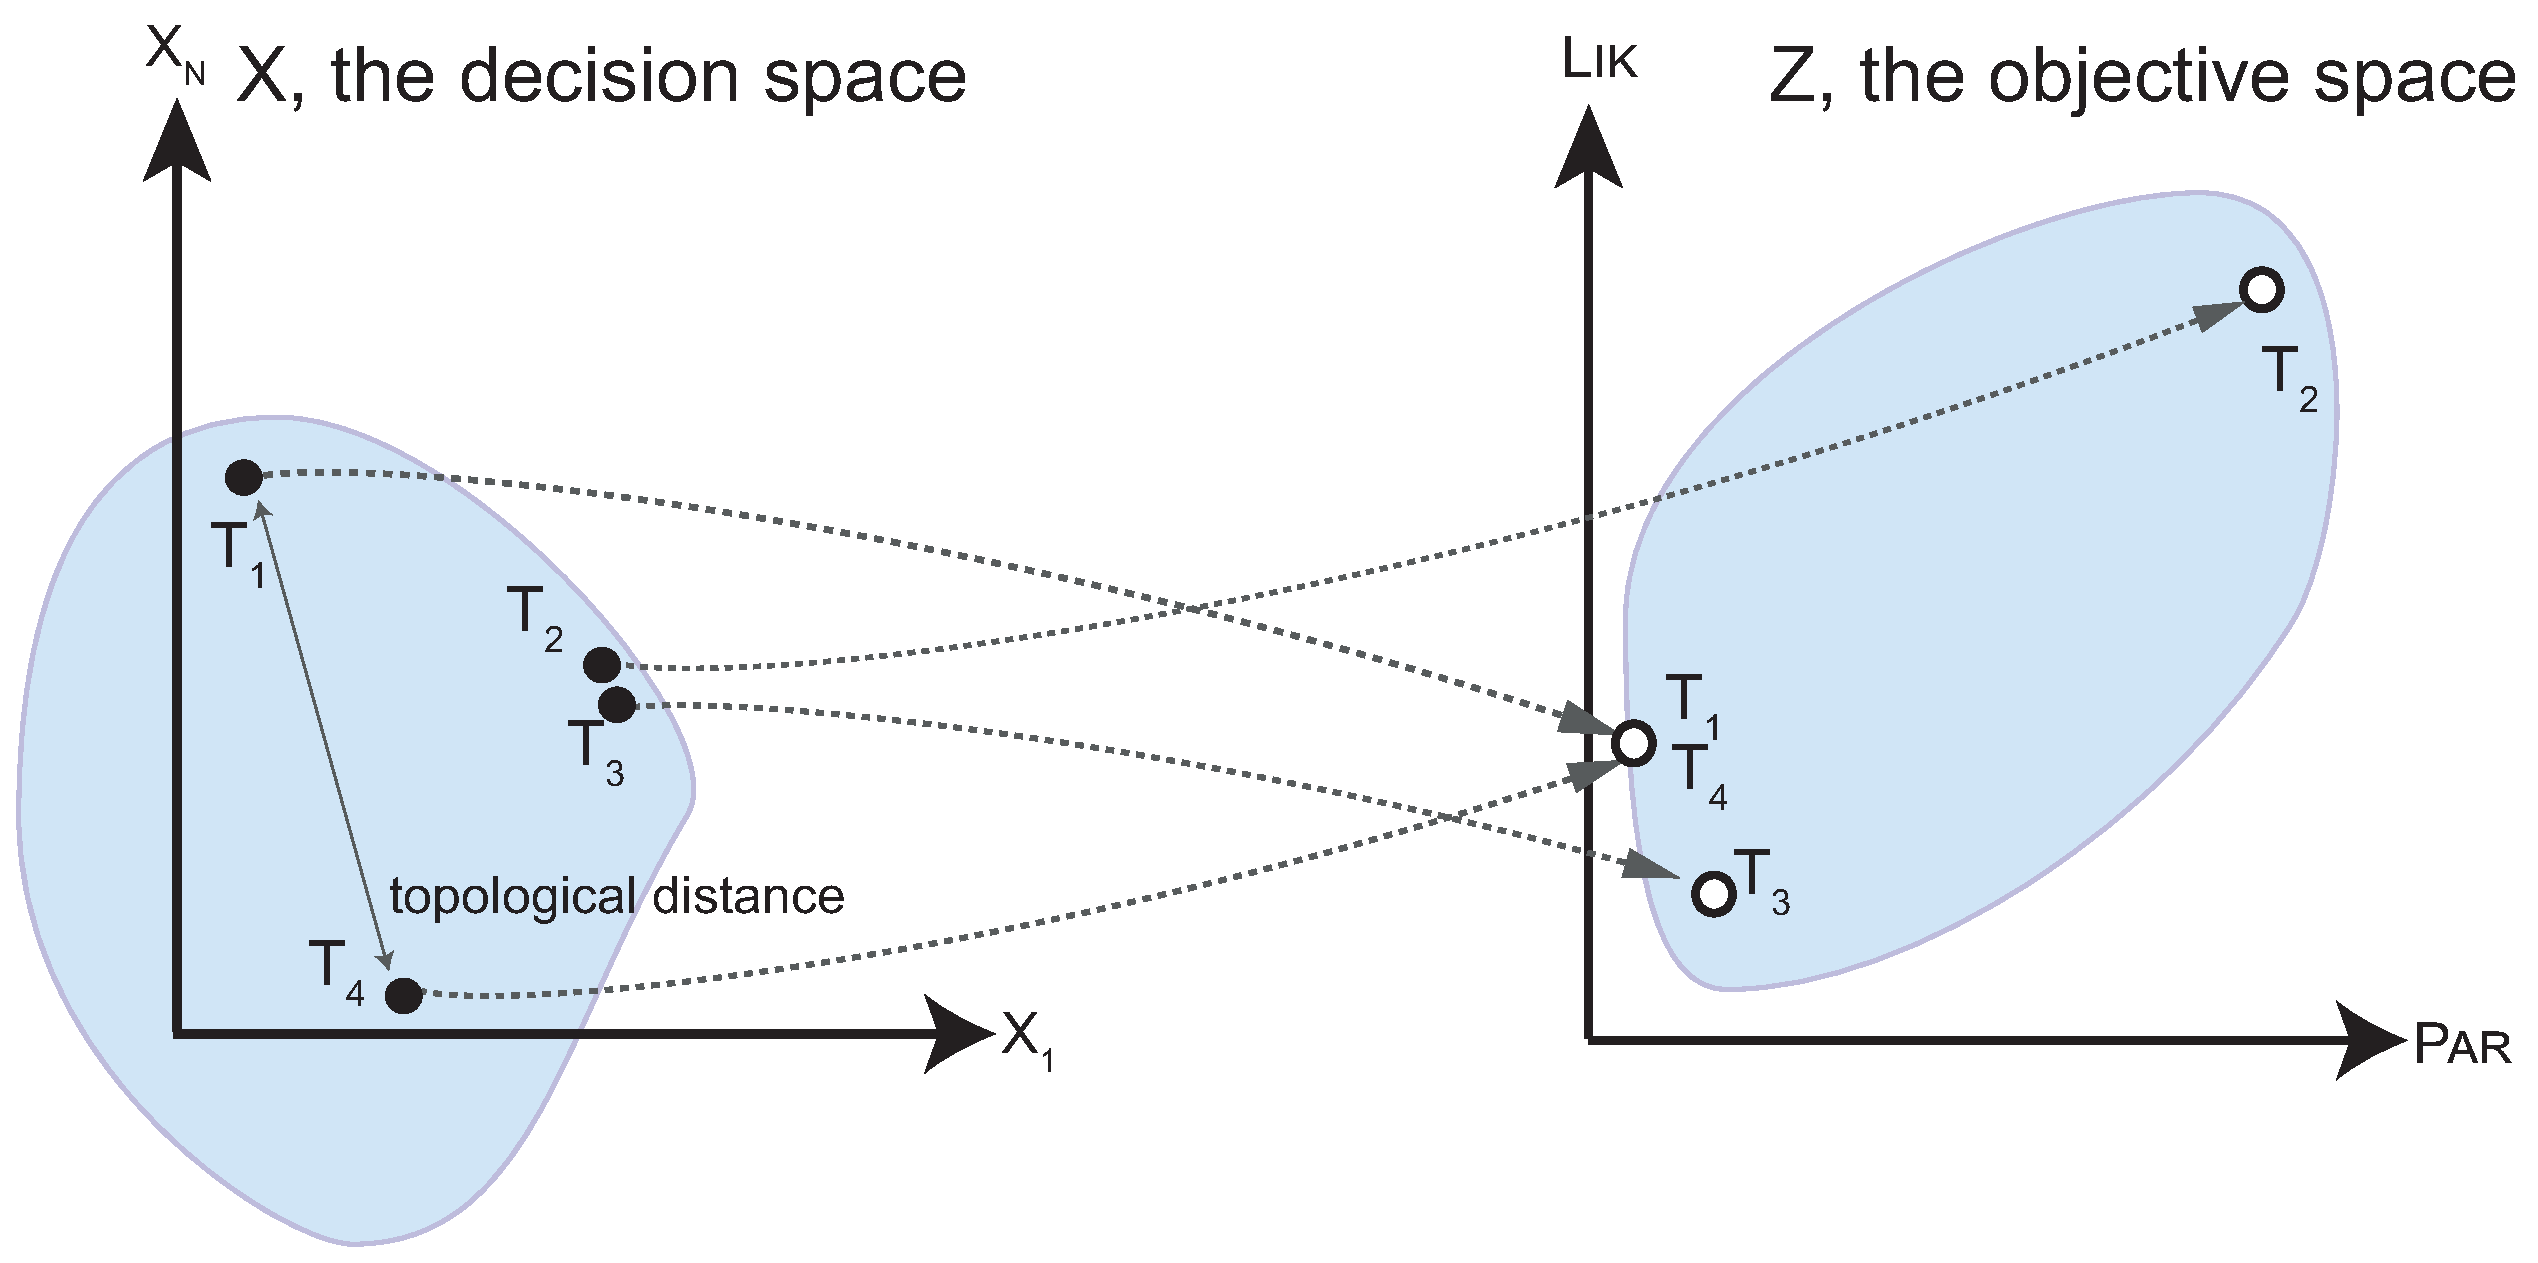
\includegraphics[scale=.3]{Images/multimodalProblem.eps}
    \caption{Relación espacio de decisiones y espacio objetivo \citep{VillalobosCid2018c}}
    \label{fig:multimodalProblem}
\end{figure}

Dentro de las diferentes propuestas multiobjetivo, el algoritmo memético (MO-MA) basado en el esquema de trabajo de NSGA-II \citep{VillalobosCid2019} tiene métricas de calidad competitivas en comparación con las estrategias multiobjetivo del estado del arte. Sin embargo, este algoritmo sigue el enfoque de optimización de los criterios utilizados para inferir. Es por ello que se propone incorporar un nuevo operador multimodal a dicho algoritmo, este debe permitir obtener información sobre las topologías de los árboles evaluados, y con ello establecer una nueva métrica de distancia topológica en el proceso de actualización de la frontera de pareto de MO-MA (Anexo \ref{subsec:mo-ma}). De esta manera se lograría que el algoritmo no descarte historias de interés solamente por el \textit{crowding distance}. Logrando así una mayor diversidad de soluciones en términos distancia topológica entre los árboles entregados.



\subsection{Impacto esperado}
\label{sec:impact}

La realización de estudio busca mejorar la diversidad de las soluciones entregadas por las actuales estrategias multiobjetivo para inferencia filogenética. Esto por medio de la creación de un nuevo operador que considera las topologías de los árboles filogenéticos presentes en el espacio de decisión. Con esto se tendrá una nueva métrica basada en la distancia topológica de los árboles a inferir. En la literatura se encuentran diversas métricas para comparar árboles filogenéticos respecto a la topología de éstos. Entre las métricas de comparación se encuentran \textit{Robinson-Foulds} \citep{Briand2020}, \textit{Path difference, Branch score} y \textit{Kendall-Colijn}, entre otros \citep{Jombart2017}. Por lo que es necesario también comparar la utilización de la nueva estrategia multiobjetivo con diferentes distancias topológicas, con la finalidad de maximizar la diversidad de soluciones sin perder la calidad de éstas en términos de \textit{hypervolumen}.


\section{Planteamiento del problema científico}
\label{cap:problemStatement}

\subsection{Revisión preliminar de la literatura}
\label{sec:preliminarLiteratureReview}

En el campo de la inferencia filogenética multiobjetivo, existen diversos referentes de la última década que aplican diferentes estrategias para optimizar los criterios utilizados en el proceso de inferencia de árboles filogenéticos. Entre los cuales está MO-ABC \citep{Santander-Jimenez2013}, iMO-ABC \citep{Santander-Jimenez2012}, IBEA \citep{Santander-Jimenez2016b}, MOEA-MC \citep{Zhang2020}, IMOBA \citep{Santander-Jimenez2016b,Arco2020}, y MO-MA \cite{VillalobosCid2019}. De la cantidad de propuestas mencionadas, MO-MA (Multi-Objective Memetic Algorithm) destaca por tener las mejores métricas de calidad en comparación con las estrategias de inferencia filogenética multiobjetivo de última generación (Anexo \ref{subsec:state-of-the-art-Results}).

MO-MA (Anexo \ref{subsec:mo-ma}) se basa en el esquema de trabajo de NSGA-II (Figura \ref{fig:nsga2}), el cual es un algoritmo genético multiobjetivo ampliamente utilizado en diferentes problemas de optimización \citep{Correa2008}. Dentro de su marco de trabajo utiliza una métrica llamada \textit{crowding distance}, la cual en el contexto de inferencia filogenética multiobjetivo es utilizada para incrementar la diversidad de soluciones de acuerdo al espacio objetivo.

\begin{figure}[hptb]
    \centering
    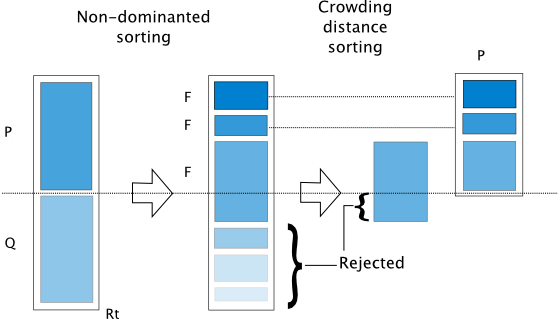
\includegraphics[scale=.9]{Images/nsga2.png}
    \caption{\textit{Elitist Non-Dominated Sorting Genetic Algorithm} \citep{Nsga2002}}
    \label{fig:nsga2}
\end{figure}


\subsection{Brecha en el conocimiento}
\label{sec:knowlegdeGap}

Investigaciones realizadas en los últimos años han demostrado que en el contexto de inferencia filogenética multiobjetivo, el espacio de decisión y el espacio objetivo no están directamente relacionados \citep{VillalobosCid2018c}. Incluso resultados obtenidos por otros estudios, sugieren que la inferencia filogenética es potencialmente multimodal \citep{Liang2016,Shi2019}. Esto quiere decir que pueden existir soluciones que a nivel topológico sean muy diferentes, sin embargo, éstas pueden converger en un mismo punto sobre el espacio objetivo. Del mismo modo, soluciones con puntos muy distantes en el espacio objetivo pueden ser muy similares en lo que a topología respecta.

En general las estrategias multiobjetivo optimizan los criterios de inferencia en son de mejorar la diversidad de las soluciones, sin embargo, no se incluye durante tal proceso información asociada a la topología de los árboles filogenéticos. En un algoritmo como MO-MA sería ideal incorporar información del espacio de decisión, con la finalidad de incrementar la diversidad de las soluciones entregadas por éste, y mantener una buena calidad de éstas.

\subsection{Preguntas de investigación}
\label{sec:researchQuestions}

\begin{itemize}
    \item ¿La incorporación de la información adicional del espacio de decisión lograría una mayor diversidad de soluciones obtenidas por MO-MA, en términos de las topologías de los árboles?
    \item ¿Cuál métrica de distancia topológica permite obtener una mayor diversidad de soluciones en términos de las topologías de los árboles filogenéticos?
\end{itemize}

\subsection{Hipótesis de trabajo}
\label{sec:hipotesis}
    
Al utilizar ciertas métricas de distancias topológicas para la incorporación de información del espacio de decisión, en el proceso de obtención de soluciones de MO-MA, se puede asegurar diversidad topologías de los árboles filogenéticos inferidos.

\section{Objetivo general y específicos del proyecto}
\label{cap:Proposal}

\subsection{Objetivo general}

Mejorar la diversidad de soluciones entregadas por un algoritmo multiobjetivo para inferencia filogenética (MO-MA), esto con la incorporación de información de las topologías de los árboles filogenéticos en el proceso inferencia.


\subsection{Objetivos específicos}

\begin{itemize}
    \item Creación de un nuevo algoritmo genético multimodal multiobjetivo que incorpore información del espacio de decisión en el proceso de inferencia filogenética.
    \item Implementar un operador multimodal que utilice distancias topológicas como métrica de diversidad.
    \item Comparar en términos de \textit{hypervolumen} la calidad de las soluciones obtenidas por el nuevo algoritmo respecto a las soluciones obtenidas por MO-MA.
    \item Realizar análisis estadístico de los resultados obtenidos por la ejecución del nuevo algoritmo con cada distancia topológica utilizada por el operador multimodal.
\end{itemize}